\documentclass[11pt,a4paper]{article}

\usepackage[utf8]{inputenc}
\usepackage[T1]{fontenc}
\usepackage{lmodern}
\usepackage[margin=2.2cm]{geometry}
\usepackage{amsmath,amssymb,amsfonts,mathtools}
\usepackage{bm}
\usepackage{booktabs}
\usepackage{array}
\usepackage{graphicx}
\usepackage{float}
\usepackage{xcolor}
\usepackage{fancyhdr}
\usepackage{titlesec}
\usepackage{hyperref}

\definecolor{amberdark}{RGB}{175, 105, 18}
\definecolor{chassisblue}{RGB}{28, 52, 84}
\definecolor{codebg}{RGB}{246, 246, 244}

\hypersetup{
    colorlinks=true,
    linkcolor=chassisblue,
    citecolor=amberdark,
    urlcolor=chassisblue,
    pdftitle={Silken Tofu: Mathematical Formulation of a Component-Level Electro-Optical Leveling Amplifier},
    pdfauthor={Studio Audio Labs}
}

\pagestyle{fancy}
\fancyhf{}
\fancyhead[L]{\small\textbf{Silken Tofu (Model LA-2A / T4B)} --- Mathematical \& Physical Whitepaper}
\fancyhead[R]{\small\thepage}
\renewcommand{\headrulewidth}{0.4pt}

\title{
    \vspace{-1.0cm}
    \textbf{\LARGE Silken Tofu: Component-Level Physical \& Mathematical Formulation of a 1965 Electro-Optical Leveling Amplifier}\\[0.5em]
    \large Coupling Destriau AC Electroluminescence, Two-Trap Semiconductor Recombination Kinetics,\\
    Oversampled Triode-Transformer Saturation, and Phase-Coherent Parallel Mixing
}
\author{
    \textbf{Kijjaz \& Studio Audio Labs}\\
    \small Technical Reference Manual \& DSP Whitepaper (\texttt{v0.0.2})
}
\date{November 2026}

\begin{document}

\maketitle

\begin{abstract}
\noindent
This document presents the complete continuous-time physical equations and discrete-time digital signal processing (DSP) formulation of \textbf{Silken Tofu}, a component-level virtual analog emulation and semiconductor-physics extension of the 1965 Teletronix LA-2A Leveling Amplifier and its T4B electro-optical attenuator cell. Unlike canonical single-pole envelope compressors, the LA-2A exhibits an implicit feedback topology coupled to a non-linear phosphor electroluminescent (EL) panel and a polycrystalline Cadmium Sulfide (CdS) photoresistor governed by multi-level carrier trapping. We formulate (1) a continuous feedback/feed-forward sidechain morphing law with negative-ratio over-compression, $R_{37}$ pre-emphasis, capacitive EL displacement current, and an empirical $100\text{ k}\Omega$ audio-taper gain law; (2) the Destriau AC electroluminescence equation with an \texttt{NE-2} neon breakdown soft knee and sub-threshold \emph{Bias Pre-Warmth}; (3) a stiff coupled two-trap semiconductor ordinary differential equation (ODE) system supporting four photoconductor chemistries (\texttt{CdS}, \texttt{CdSe}, \texttt{Aged 50Y CdS}, and \texttt{Silicon Photodiode}) plus negative trap memory (\emph{Optical Bloom}); (4) a polyphase oversampled ($1\times/2\times/4\times/8\times$) vacuum tube and transformer signal path modeling \texttt{UTC HA-100X} Permalloy hysteresis, dynamic \texttt{12AX7A} Miller capacitance, Koren triode plate curves with $C_2$ grid-conduction bias shift, shared $275\text{ V B+}$ RC power supply sag, and a \texttt{12BH7A} White Cathode Follower driving a \texttt{UTC A-24} transformer; and (5) a phase-coherent parallel Dry/Wet architecture that eliminates all three sources of parallel comb filtering and sub-bass phase cancellation.
\end{abstract}

\tableofcontents
\vspace{0.8em}
\hrule
\vspace{1.2em}

% ============================================================================
\section{System Architecture \& Signal Flow}
% ============================================================================

In the historical 1965 Teletronix LA-2A circuit, the input audio traverses an input transformer (\texttt{UTC HA-100X}) to a voltage divider formed by a series $68\text{ k}\Omega$ resistor ($R_6$) and the T4B's main audio-path Cadmium Sulfide (CdS) photoresistor ($R_{\text{LDR}}$) shunted to ground. The attenuated voltage at the divider node drives the grid of the first \texttt{12AX7A} voltage amplifier stage ($V_1$), followed by a \texttt{12BH7A} White Cathode Follower ($V_2$) and the \texttt{UTC A-24} output transformer. Crucially, the sidechain amplifier (\texttt{12AX7A} + \texttt{6AQ5} pentode) taps the signal \emph{after} the T4B voltage divider, creating a closed-loop feedback control system.

\begin{figure}[H]
    \centering
    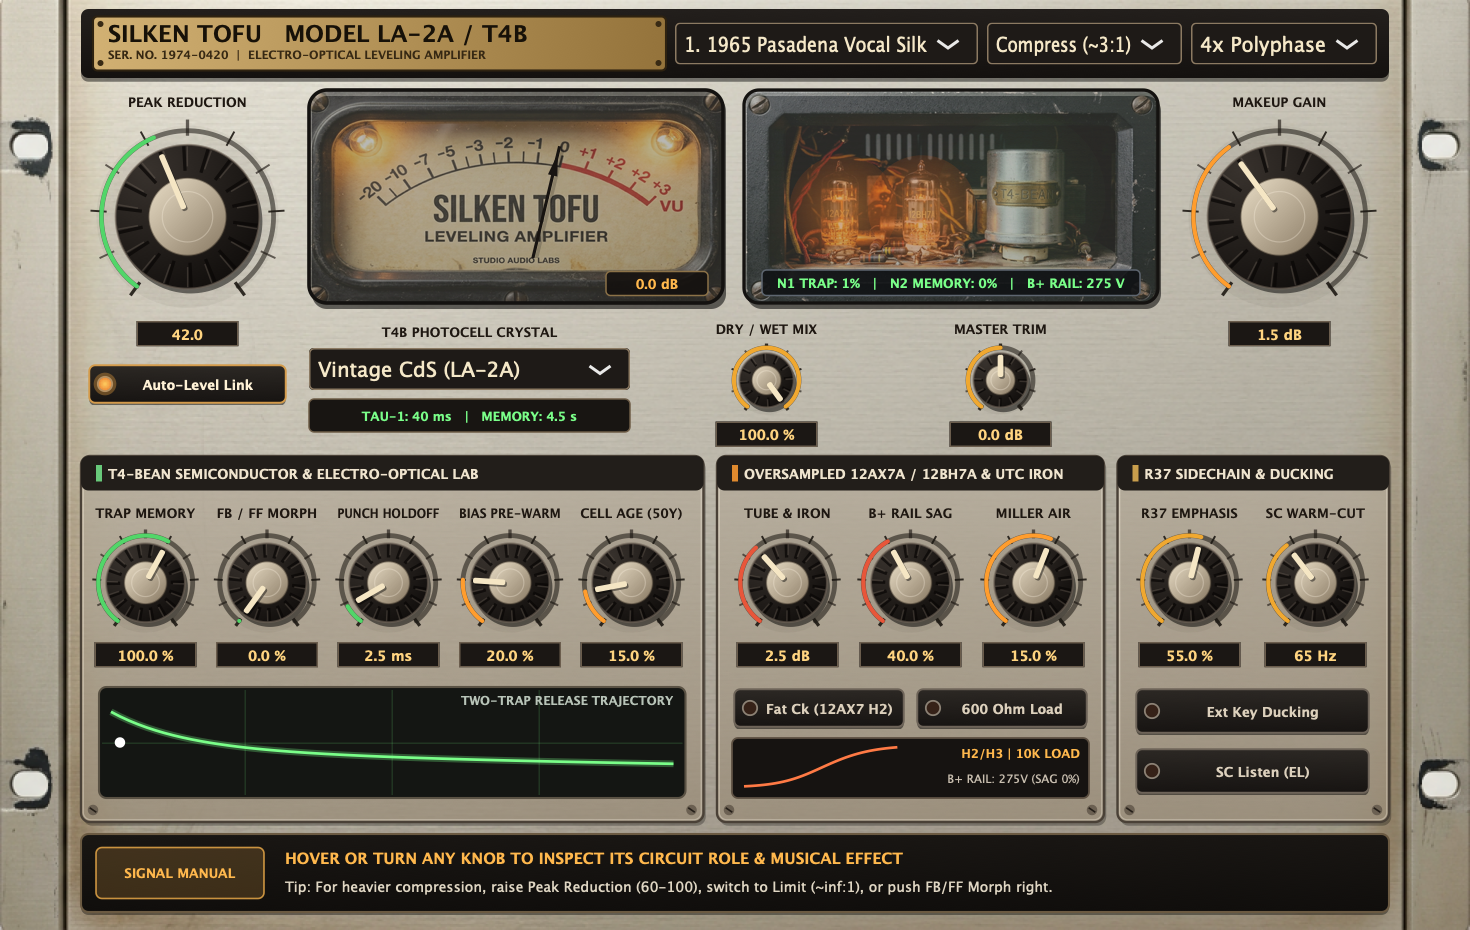
\includegraphics[width=0.96\textwidth]{figures/silken_tofu_v002_ui.png}
    \caption{The \textbf{Silken Tofu} (\texttt{v0.0.2}) front panel, showing the main Peak Reduction and Makeup Gain controls, illuminated VU and T4B X-Ray telemetry windows, and the three laboratory expansion cards.}
    \label{fig:ui}
\end{figure}

Let $f_s$ denote the host sample rate (e.g., $44.1\text{ kHz}$ to $192\text{ kHz}$) and $M \in \{1, 2, 4, 8\}$ denote the user-selectable polyphase oversampling factor. The effective internal sampling rate is:
\begin{equation}
    f_{\text{os}} = M \, f_s, \qquad T_s = \frac{1}{f_{\text{os}}}.
\end{equation}
All continuous-time state integrators scale explicitly with $T_s$ or the normalized sample-rate ratio $\rho_s = 44100 / f_{\text{os}}$ to guarantee strict sample-rate invariance across $44.1\text{ kHz}$, $48\text{ kHz}$, $88.2\text{ kHz}$, and $96\text{ kHz}$.

% ============================================================================
\section{Stage 1: Sidechain Topology, Pre-Emphasis \& Audio-Taper Law}
% ============================================================================

\subsection{Continuous Feedback / Feed-Forward Morphing \& Negative Ratios}

Let $x_{\text{in}}[n]$ be the stereo-linked mono input sample (or external key input $x_{\text{key}}[n]$ when \textbf{Ext Key Ducking} is engaged), and let $y_{\text{div}}[n-1] = G_{\text{T4B}}[n-1]\,x_{\text{in}}[n-1]$ be the one-sample-delayed output of the T4B resistive voltage divider. The \textbf{FB / FF Morph} parameter $m_{\text{ff}} \in [0\%, 125\%]$ defines a normalized blending coefficient $\alpha_{\text{ff}} = m_{\text{ff}} / 100 \in [0, 1.25]$:
\begin{equation}
    x_{\text{sc,raw}}[n] = (1 - \alpha_{\text{ff}})\,y_{\text{div}}[n-1] + \alpha_{\text{ff}}\,x_{\text{key}}[n].
    \label{eq:fb_ff_morph}
\end{equation}
The steady-state compression slope follows directly from Eq.~\eqref{eq:fb_ff_morph}:
\begin{itemize}
    \item \textbf{Pure Feedback ($\alpha_{\text{ff}} = 0$):} The sidechain sees only the compressed divider node $y_{\text{div}}$, yielding the classic vintage LA-2A soft-knee leveling curve ($\approx 3\!:\!1$ in \texttt{Compress} mode, $\approx 10\!:\!1$ in \texttt{Limit} mode).
    \item \textbf{Pure Feed-Forward ($\alpha_{\text{ff}} = 1.0$):} The sidechain is driven purely by the uncompressed input $x_{\text{key}}$, producing hard feed-forward limiting where higher input levels force $R_{\text{LDR}} \to R_{\text{min}}$ without feedback self-regulation.
    \item \textbf{Over-Biased Feed-Forward ($\alpha_{\text{ff}} \in (1.0, 1.25]$):} In Eq.~\eqref{eq:fb_ff_morph}, $(1-\alpha_{\text{ff}}) < 0$, subtracting a fraction of the compressed signal from the feed-forward drive and creating an aggressive negative-ratio over-compression curve above threshold.
\end{itemize}

\subsection{Sidechain Warm-Cut High-Pass \& \texorpdfstring{$R_{37}$}{R37} Pre-Emphasis Filter}

To prevent low-frequency bass energy from over-triggering the EL panel, the sidechain incorporates a first-order high-pass filter (\textbf{SC Warm-Cut}) with cutoff frequency $f_{\text{hp}} \in [20, 400]\text{ Hz}$. With pole coefficient $a_{\text{hp}} = \exp(-2\pi f_{\text{hp}} T_s)$, the low-pass state $s_{\text{hp}}[n]$ and high-passed signal $x_{\text{hp}}[n]$ are:
\begin{align}
    s_{\text{hp}}[n] &= a_{\text{hp}}\,s_{\text{hp}}[n-1] + (1 - a_{\text{hp}})\,x_{\text{sc,raw}}[n], \\
    x_{\text{hp}}[n] &= x_{\text{sc,raw}}[n] - s_{\text{hp}}[n].
\end{align}

Next, the historical LA-2A features trimmer potentiometer $R_{37}$ (\textbf{R37 Emphasis}), which adjusts a shelving RC network in the \texttt{12AX7A} sidechain amplifier stage. Let $r_{37} \in [0, 1]$ be the normalized $R_{37}$ emphasis control ($0\%$ = flat broadcast setting, $45\%$ = factory stock calibration, $100\%$ = heavy HF de-essing). Using a corner frequency $f_{r37} = 1800\text{ Hz}$ and pole $a_{r37} = \exp(-2\pi f_{r37} T_s)$:
\begin{align}
    s_{r37}[n] &= a_{r37}\,s_{r37}[n-1] + (1 - a_{r37})\,x_{\text{hp}}[n], \\
    x_{r37}[n] &= x_{\text{hp}}[n] + 2.8\,r_{37}\,\bigl(x_{\text{hp}}[n] - s_{r37}[n]\bigr).
\end{align}

\subsection{Capacitive EL Panel Displacement Current}

Because the T4B electroluminescent panel is physically a lossy parallel-plate capacitor ($C_{\text{EL}} \approx 2.2\text{ nF}$ in parallel with a non-linear phosphor conductance), its instantaneous displacement current is proportional to the time derivative of the applied voltage:
\begin{equation}
    i_{\text{disp}}(t) = C_{\text{EL}}\,\frac{dv_{\text{EL}}(t)}{dt}.
\end{equation}
In discrete time, we model this high-frequency luminescent boost by adding a scaled backward difference normalized by $\rho_s^{-1} = f_{\text{os}} / 44100$:
\begin{equation}
    x_{\text{el}}[n] = x_{r37}[n] + 0.18\,\frac{f_{\text{os}}}{44100}\,\bigl(x_{r37}[n] - x_{r37}[n-1]\bigr).
\end{equation}

\subsection{\texorpdfstring{$100\text{ k}\Omega$}{100 kOhm} Audio-Taper Peak Reduction Law \& Full-Wave Peak Bridge}

On vintage hardware, the \textbf{Peak Reduction} dial is a $100\text{ k}\Omega$ logarithmic/audio-taper potentiometer feeding the grid of the sidechain amplifier. To provide smooth vocal control across $0\text{--}50$ while delivering massive gain reduction on modern $-25\text{ to }-14\text{ dBFS}$ mixes at settings $60\text{--}100$, the normalized parameter $p \in [0, 1]$ is mapped via a three-region polynomial-exponential law:
\begin{equation}
    G_{\text{PR}}(p) = 3.2\,p + 8.5\,p^{2.6} + 14.0\,\max(0,\,p - 0.55)^{3.0}.
    \label{eq:pr_taper}
\end{equation}
Notice that at $p = 0.5$, $G_{\text{PR}}(0.5) = 3.00$, whereas at $p = 1.0$, $G_{\text{PR}}(1.0) = 12.98$, providing an extra $+12.7\text{ dB}$ of sidechain drive in the upper half of the dial. The instantaneous rectified sidechain voltage (scaled to the \texttt{6AQ5} pentode plate swing) is:
\begin{equation}
    V_{\text{inst}}[n] = 95.0 \, G_{\text{PR}}(p) \, \bigl|x_{\text{el}}[n]\bigr|.
\end{equation}

To bridge the zero-crossings of low-frequency audio cycles without erasing the natural AC ripple that modulates the EL panel, $V_{\text{inst}}[n]$ passes through an asymmetric peak bridge with a $0.15\text{ ms}$ attack and an $18.0\text{ ms}$ inter-cycle hold decay:
\begin{equation}
    V_{\text{ac}}[n] = a_{\text{ac}}\,V_{\text{ac}}[n-1] + (1 - a_{\text{ac}})\,V_{\text{inst}}[n], \qquad
    a_{\text{ac}} = \begin{cases}
        \exp\!\left(-\dfrac{T_s}{0.00015}\right), & V_{\text{inst}}[n] > V_{\text{ac}}[n-1], \\[1.0em]
        \exp\!\left(-\dfrac{T_s}{0.01800}\right), & V_{\text{inst}}[n] \le V_{\text{ac}}[n-1].
    \end{cases}
\end{equation}

Finally, the \textbf{Punch Holdoff} parameter $\tau_{\text{punch}} \in [0, 30]\text{ ms}$ introduces an optional pre-luminescence low-pass filter that delays initial photon emission so drum transients punch through before the T4B cell clamps down:
\begin{equation}
    V_{\text{sc}}[n] = \begin{cases}
        a_{\text{punch}}\,V_{\text{sc}}[n-1] + (1 - a_{\text{punch}})\,V_{\text{ac}}[n], & \tau_{\text{punch}} > 0.05\text{ ms}, \\
        V_{\text{ac}}[n], & \text{otherwise},
    \end{cases}
    \qquad a_{\text{punch}} = \exp\!\left(-\frac{T_s}{\tau_{\text{punch}}}\right).
\end{equation}

% ============================================================================
\section{Stage 2: Destriau AC Electroluminescence \& \texttt{NE-2} Neon Clamp}
% ============================================================================

\subsection{Sub-Threshold Bias Pre-Warmth \& \texttt{NE-2} Breakdown Soft Knee}

In the T4B module, the ZnS:Cu electroluminescent panel exhibits a dead-zone threshold voltage $V_0$ below which practically zero photons are emitted. The \textbf{Bias Pre-Warm} parameter $b \in [0, 1]$ injects a sub-threshold quiescent AC bias voltage $V_{\text{bias}} = 0.88\,b\,V_0$ summed in quadrature (RMS power addition) with the sidechain drive $V_{\text{sc}}$:
\begin{equation}
    V_{\text{eff}}[n] = \sqrt{V_{\text{sc}}^2[n] + (0.88\,b\,V_0)^2},
\end{equation}
where the threshold parameter $V_0$ depends on the \textbf{Compress / Limit} mode switch ($R_{25}$ screen-grid voltage divider on the \texttt{6AQ5} pentode):
\begin{equation}
    V_0 = \begin{cases}
        19.0\text{ V}, & \text{\texttt{Compress} mode } (\approx 3\!:\!1), \\
        15.0\text{ V}, & \text{\texttt{Limit} mode } (\approx 10\!:\!1 \text{ to } \infty\!:\!1).
    \end{cases}
\end{equation}

In parallel with the EL panel sits an \texttt{NE-2} neon gas-discharge bulb that fires around $V_{\text{clamp}} = 55.0\text{ V}$ to regulate high-voltage excursions and define the compression knee:
\begin{equation}
    V_{\text{clamped}}[n] = \begin{cases}
        V_{\text{eff}}[n], & V_{\text{eff}}[n] \le V_{\text{clamp}}, \\[0.5em]
        V_{\text{clamp}} + 35.0\,\tanh\!\left(\dfrac{V_{\text{eff}}[n] - V_{\text{clamp}}}{35.0}\right), & V_{\text{eff}}[n] > V_{\text{clamp}}.
    \end{cases}
\end{equation}

\subsection{Destriau Law of Phosphor Luminescence}

Following Destriau's physical law for AC powder electroluminescence via impact ionization across copper-doped zinc sulfide (ZnS:Cu) crystallite barriers, the normalized photon flux $L[n]$ is zero for $V_{\text{clamped}}[n] \le 0.85\,V_0$, and for $V_{\text{clamped}}[n] > 0.85\,V_0$ is governed by:
\begin{equation}
    L(V_{\text{clamped}}, \alpha_{\text{age}}) = (1 - 0.18\,\alpha_{\text{age}}) \left(\frac{V_{\text{clamped}}}{V_0}\right)^{\!\gamma} \exp\!\left(-\frac{V_0}{V_{\text{clamped}} - 0.82\,V_0}\right),
    \label{eq:destriau}
\end{equation}
where $\alpha_{\text{age}} \in [0, 1]$ is the normalized \textbf{Cell Age (50Y)} parameter modeling phosphor half-life degradation over decades of studio operation, and the exponent $\gamma$ is set by the \textbf{Compress / Limit} switch:
\begin{equation}
    \gamma = \begin{cases}
        1.55, & \text{\texttt{Compress} mode}, \\
        2.15, & \text{\texttt{Limit} mode}.
    \end{cases}
\end{equation}

\begin{figure}[H]
    \centering
    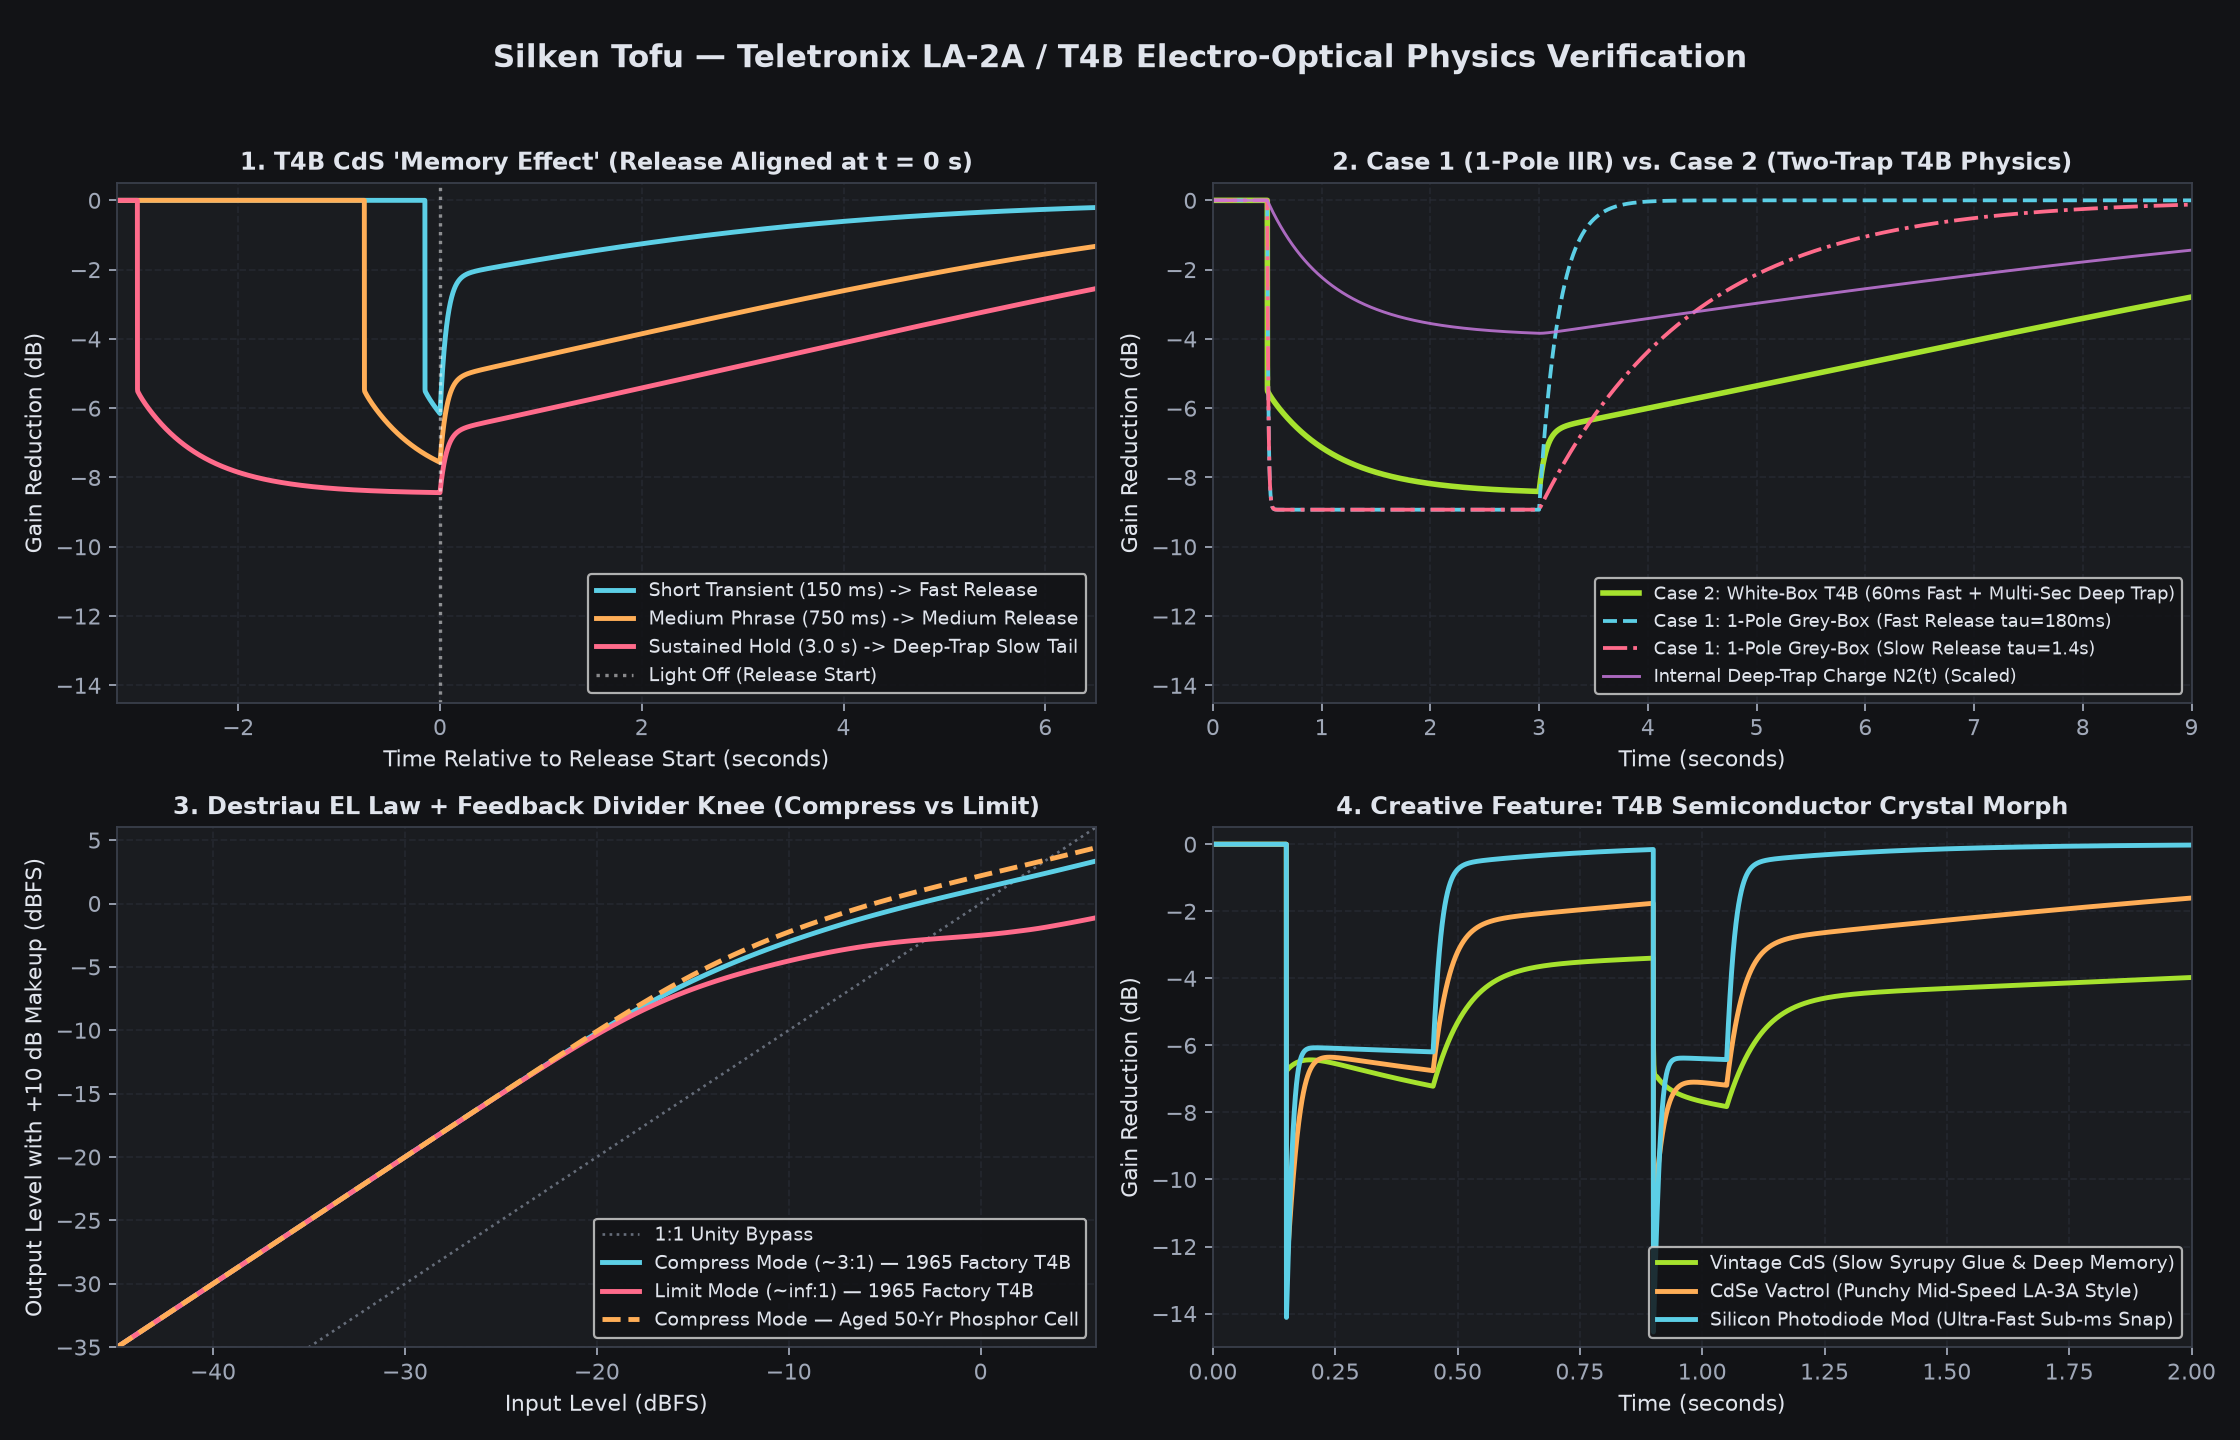
\includegraphics[width=0.98\textwidth]{figures/silken_tofu_t4b_physics.png}
    \caption{Physical verification of the T4-Bean electro-optical model: (Top-Left) Destriau luminescence curve $L(V)$ showing the sub-threshold dead-zone and \texttt{Compress} vs.\ \texttt{Limit} slopes; (Top-Right) program-dependent two-stage release recovery after $0.1\text{ s}$, $0.5\text{ s}$, $2.0\text{ s}$, and $5.0\text{ s}$ exposure durations; (Bottom-Left) step response comparison across all four selectable cell chemistries; (Bottom-Right) Negative Trap Memory (\emph{Optical Bloom}) producing an upward gain swell on release.}
    \label{fig:t4b_physics}
\end{figure}

% ============================================================================
\section{Stage 3: Two-Trap Semiconductor Carrier Recombination ODEs}
% ============================================================================

\subsection{Physical Origin of the Program-Dependent LA-2A Release}

In polycrystalline II-VI semiconductors such as Cadmium Sulfide (CdS) and Cadmium Selenide (CdSe), incident photons with energy $h\nu > E_g$ excite electrons from the valence band into the conduction band, increasing free carrier density and lowering cell resistance. However, crystal lattice defects and impurities introduce two distinct distributions of localized energy states within the forbidden bandgap:
\begin{enumerate}
    \item \textbf{Shallow Recombination Centers ($N_1$):} Equilibrate rapidly with the conduction band ($\tau_{r1} \approx 35\text{--}60\text{ ms}$), governing the fast initial recovery after transient peaks.
    \item \textbf{Deep Electron Traps ($N_2$):} Capture electrons slowly during sustained illumination and thermally re-emit them over several seconds ($\tau_{r2} \approx 0.6\text{--}5.0\text{ s}$) according to a non-linear, occupancy-dependent rate.
\end{enumerate}

Table~\ref{tab:cell_models} summarizes the baseline physical parameters for the four selectable \textbf{Cell Models} in Silken Tofu, which are further modulated in real time by the continuous \textbf{Cell Age (50Y)} control $\alpha_{\text{age}} \in [0, 1]$.

\begin{table}[H]
\centering
\caption{Baseline Semiconductor Parameters Across Selectable T4-Bean Photoconductor Models}
\label{tab:cell_models}
\vspace{0.3em}
\resizebox{\textwidth}{!}{%
\begin{tabular}{@{}lcccccc@{}}
\toprule
\textbf{Cell Chemistry Model} & $\tau_{a0}$ (ms) & $\tau_{r1}$ (ms) & $\tau_{r2,0}$ (s) & $k_{\text{trap}}$ ($\text{s}^{-1}$) & $\mu$ (Gamma) & $R_{\text{dark}}$ ($\text{M}\Omega$) \\
\midrule
1. \textbf{Vintage 1968 CdS (T4B)} & $11.5\,(1 - 0.25\alpha_{\text{age}})$ & $58.0$ & $1.15\,(1 + 0.8\alpha_{\text{age}})$ & $1.85$ & $0.88 + 0.14\alpha_{\text{age}}$ & $1.5\,(1 - 0.65\alpha_{\text{age}})$ \\
2. \textbf{Aged 50-Year CdS (Fatigued)} & $8.2$ & $75.0$ & $2.10$ & $2.60$ & $1.04$ & $0.45$ \\
3. \textbf{CdSe Vactrol (LA-3A Style)} & $3.2$ & $32.0$ & $0.55$ & $1.10$ & $0.96$ & $1.50$ \\
4. \textbf{Fast Silicon Photodiode} & $0.8$ & $18.0$ & $0.12$ & $0.25$ & $0.78$ & $1.50$ \\
\bottomrule
\end{tabular}%
}
\end{table}

\subsection{Coupled Differential Equations for \texorpdfstring{$N_1(t)$}{N1(t)} and \texorpdfstring{$N_2(t)$}{N2(t)}}

Let $\Phi(L) = L^{0.92}$ denote the effective photo-carrier generation target. Under high photon flux $L$, carrier generation accelerates due to space-charge barrier lowering, reducing the effective attack time constant $\tau_a(L)$:
\begin{equation}
    \tau_a(L) = \frac{\tau_{a0}}{1 + 4.5\,L^{0.85}}.
\end{equation}
The shallow carrier concentration $N_1(t)$ obeys the state-dependent first-order ODE:
\begin{equation}
    \frac{dN_1(t)}{dt} = \frac{\Phi(L) - N_1(t)}{\tau_1(L, N_1)}, \qquad
    \tau_1(L, N_1) = \begin{cases}
        \tau_a(L), & \Phi(L) > N_1(t) \quad (\text{Attack}), \\[0.4em]
        \tau_{r1}, & \Phi(L) \le N_1(t) \quad (\text{Fast Release}).
    \end{cases}
    \label{eq:ode_n1}
\end{equation}

Simultaneously, the deep trap occupancy $N_2(t)$ couples to $N_1(t)$ with asymmetric capture and thermal emission kinetics:
\begin{equation}
    \frac{dN_2(t)}{dt} = \begin{cases}
        k_{\text{trap}}\,\bigl(N_1(t) - N_2(t)\bigr), & N_1(t) > N_2(t) \quad (\text{Deep Trapping}), \\[0.6em]
        \dfrac{N_1(t) - N_2(t)}{\tau_{r2}(N_2, m_{\text{trap}})}, & N_1(t) \le N_2(t) \quad (\text{Slow Thermal Release}),
    \end{cases}
    \label{eq:ode_n2}
\end{equation}
where $m_{\text{trap}} \in [-0.5, 2.0]$ is the normalized \textbf{Trap Memory} parameter ($-50\%$ to $+200\%$), and the history-dependent slow release time constant increases with deep-trap saturation:
\begin{equation}
    \tau_{r2}(N_2, m_{\text{trap}}) = \tau_{r2,0}\,\Bigl(1 + 6.5\,\max(0, m_{\text{trap}})\,\min\bigl(N_2(t),\,1.5\bigr)\Bigr).
\end{equation}
Both Eq.~\eqref{eq:ode_n1} and Eq.~\eqref{eq:ode_n2} are integrated unconditionally reliably at every oversampled step using exact exponential Euler integration:
\begin{align}
    N_1[n] &= \Phi[n] + \bigl(N_1[n-1] - \Phi[n]\bigr)\,\exp\!\left(-\frac{T_s}{\tau_1[n]}\right), \\
    N_2[n] &= N_1[n] + \bigl(N_2[n-1] - N_1[n]\bigr)\,\exp\!\left(-r_2[n]\,T_s\right),
\end{align}
where $r_2[n] = k_{\text{trap}}$ during capture ($N_1[n] > N_2[n-1]$) and $r_2[n] = 1 / \tau_{r2}[n]$ during thermal release.

\subsection{Photoconductor Resistance Law \& Negative Trap Memory (\emph{Optical Bloom})}

The instantaneous photoresistor resistance $R_{\text{LDR}}[n]$ combines dark resistance $R_{\text{dark}}$ with the weighted carrier densities $N_1[n]$ and $N_2[n]$. Crucially, Silken Tofu extends $m_{\text{trap}}$ into the negative domain $[-0.5, 0)$:
\begin{itemize}
    \item \textbf{Positive Trap Memory ($m_{\text{trap}} \ge 0$):} Deep traps contribute positively to conductivity with weight $\kappa(m_{\text{trap}}) = 24.0\,m_{\text{trap}}$, holding $R_{\text{LDR}}$ low after sustained loud passages (the classic multi-second LA-2A release tail).
    \item \textbf{Negative Trap Memory / Optical Bloom ($m_{\text{trap}} < 0$):} Deep traps act as temporary carrier-depletion centers ($\kappa(m_{\text{trap}}) = 16.0\,m_{\text{trap}} < 0$) once the primary shallow carriers $N_1[n]$ recombine, causing $R_{\text{LDR}}$ to momentarily overshoot above its steady-state trajectory and producing a musical upward ``swell'' or bloom after transient hits.
\end{itemize}
Defining the effective carrier sum:
\begin{equation}
    C_{\text{eff}}[n] = \max\!\Bigl(0.02,\; 1.0 + 38.0\,N_1[n] + \kappa(m_{\text{trap}})\,N_2[n]\Bigr),
\end{equation}
the photoresistor impedance and the resulting T4B voltage divider gain across the series resistor $R_6 = 68\text{ k}\Omega$ are:
\begin{equation}
    R_{\text{LDR}}[n] = R_{\text{dark}} + (R_{\text{min}} - R_{\text{dark}})\left(1 - C_{\text{eff}}[n]^{-\mu}\right), \qquad
    G_{\text{T4B}}[n] = \frac{R_{\text{LDR}}[n]}{R_6 + R_{\text{LDR}}[n]},
    \label{eq:t4b_divider}
\end{equation}
clipped safely to $R_{\text{LDR}}[n] \in [R_{\text{min}}, R_{\text{dark}}]$ with $R_{\text{min}} = 120\text{ }\Omega$.

\begin{figure}[H]
    \centering
    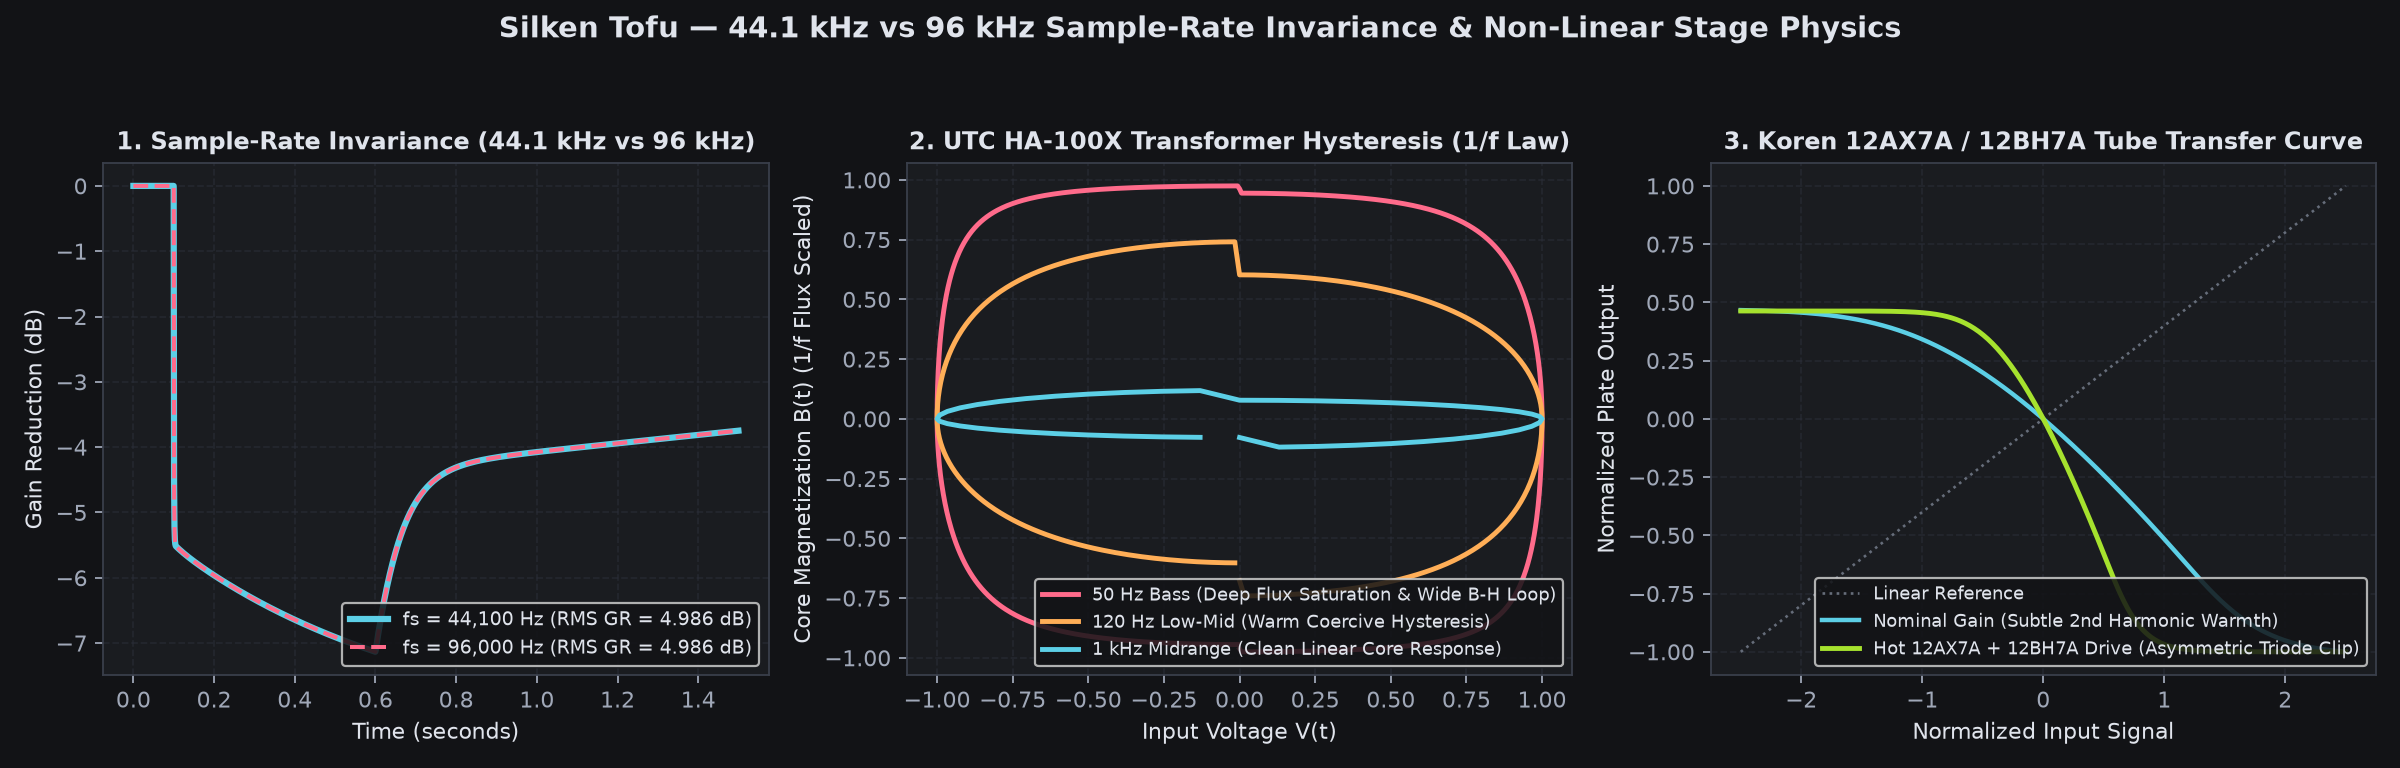
\includegraphics[width=0.98\textwidth]{figures/silken_tofu_circuit_stages.png}
    \caption{Circuit-stage characteristics: (Top-Left) Steady-state compression curves across \textbf{FB / FF Morph} settings from $0\%$ (Feedback) to $125\%$ (Negative-Ratio Over-Compression); (Top-Right) $R_{37}$ sidechain pre-emphasis frequency responses; (Bottom-Left) Gain-reduction-dependent \texttt{12AX7A} Miller capacitance high-frequency roll-off; (Bottom-Right) Harmonic spectrum of the \texttt{12AX7A} / \texttt{12BH7A} tube stage showing the $+5.7\text{ dB}$ increase in 2nd-harmonic warmth ($H_2$) when engaging \textbf{Fat Ck}.}
    \label{fig:circuit_stages}
\end{figure}

% ============================================================================
\section{Stage 4: Oversampled Vacuum Tube \& Transformer Signal Path}
% ============================================================================

To suppress harmonic aliasing from the triode stages and transformer core saturation, the entire audio path runs inside a selectable $1\times / 2\times / 4\times / 8\times$ polyphase half-band IIR oversampler (\texttt{juce::dsp::Oversampling::filterHalfBandPolyphaseIIR}).

\subsection{\texttt{UTC HA-100X} Input Transformer Hysteresis (\texorpdfstring{$1/f$}{1/f} Flux Integrator)}

The magnetic core flux $\Phi_{\text{core}}(t)$ of the \texttt{UTC HA-100X} nickel-iron (Permalloy) input transformer is the time integral of the primary voltage, meaning core saturation varies inversely with frequency ($\Phi_{\text{core}} \propto V / f$) and concentrates harmonic generation below $150\text{ Hz}$. We model this via a leaky flux integrator with corner frequency $f_{\text{leak}} = 28\text{ Hz}$ and excitation scaling $f_{\text{xfmr}} = 55\text{ Hz}$:
\begin{equation}
    \Phi_{\text{core}}[n] = e^{-2\pi f_{\text{leak}} T_s}\,\Phi_{\text{core}}[n-1] + 2\pi f_{\text{xfmr}} T_s\,x_{\text{in}}[n].
\end{equation}
Using a simplified Jiles-Atherton magnetic hysteresis pinning term driven by the flux derivative $\Delta \Phi_{\text{core}}[n] = \Phi_{\text{core}}[n] - \Phi_{\text{core}}[n-1]$:
\begin{equation}
    \Phi_{\text{hyst}}[n] = \Phi_{\text{core}}[n] - 0.15\,d_{\text{tube}}\,\operatorname{sgn}\!\bigl(\Delta\Phi_{\text{core}}[n]\bigr)\Bigl(1 - e^{-|\Phi_{\text{core}}[n]|}\Bigr),
\end{equation}
where $d_{\text{tube}} \in [0, 1]$ is the normalized \textbf{Tube \& Iron} drive parameter. The transformer output fed into the T4B attenuator divider is:
\begin{equation}
    v_{\text{xfmr}}[n] = x_{\text{in}}[n] + 0.22\,d_{\text{tube}}\Bigl[\tanh\!\bigl(1.35\,\Phi_{\text{hyst}}[n]\bigr) - 1.35\,\Phi_{\text{core}}[n]\Bigr], \qquad
    y_{\text{div}}[n] = G_{\text{T4B}}[n]\,v_{\text{xfmr}}[n].
\end{equation}

\subsection{Dynamic \texttt{12AX7A} Miller Capacitance High-Frequency Tilt}

Because the T4B voltage divider output resistance $R_{\text{th}} = (R_6 \parallel R_{\text{LDR}})$ varies with illumination and drives the input grid of the high-mu \texttt{12AX7A} triode ($A_v \approx 60$, grid-to-plate capacitance $C_{gp} \approx 1.7\text{ pF}$), the effective Miller input capacitance $C_{\text{Miller}} = C_{gk} + C_{gp}(1 + A_v)$ forms a gain-dependent low-pass filter. Let $m_{\text{air}} \in [-1, +1]$ be the normalized \textbf{Miller Air} control ($-100\%$ dark vintage roll-off to $+100\%$ presence compensation) and $s_{\text{miller}}[n]$ be a first-order low-pass state at $f_{\text{miller}} = 4800\text{ Hz}$:
\begin{align}
    s_{\text{miller}}[n] &= a_{\text{miller}}\,s_{\text{miller}}[n-1] + (1 - a_{\text{miller}})\,y_{\text{div}}[n], \qquad a_{\text{miller}} = e^{-2\pi (4800) T_s}, \\
    v_{\text{grid1}}[n] &= y_{\text{div}}[n] + \Bigl(0.45\,m_{\text{air}} - 0.16\,\bigl(1 - G_{\text{T4B}}[n]\bigr)\Bigr)\bigl(y_{\text{div}}[n] - s_{\text{miller}}[n]\bigr).
\end{align}

\subsection{\texttt{V1 (12AX7A)} Koren Triode Model, \texorpdfstring{$C_2$}{C2} Grid Conduction \& \textbf{Fat Ck} Switch}

Let $D = 0.08 + 1.85\,d_{\text{tube}}^{1.25}$ denote the tube stage drive scalar. The static cathode bias of the \texttt{12AX7A} stage depends on whether the cathode resistor $R_9$ ($1.2\text{ k}\Omega$) is bypassed by a cathode capacitor (\textbf{Fat Ck} engaged, yielding higher asymmetric 2nd-harmonic $H_2$ warmth) or left unbypassed (stock Teletronix negative local feedback):
\begin{equation}
    V_{\text{bias}} = \begin{cases}
        -0.92\text{ V}, & \text{\textbf{Fat Ck} engaged}, \\
        -1.25\text{ V}, & \text{\textbf{Fat Ck} disengaged (stock)}.
    \end{cases}
\end{equation}
When positive peaks drive the grid-to-cathode voltage $v_{gk}[n] = D\,v_{\text{grid1}}[n] + V_{\text{bias}} - V_{C2}[n-1]$ above the grid-current conduction threshold $V_{gk,\text{thresh}} = -0.25\text{ V}$, grid electrons charge the coupling capacitor $C_2$ ($\tau_{\text{charge}} = 1.5\text{ ms}$) and discharge slowly through the grid-leak resistor ($\tau_{\text{rel}} = 45.0\text{ ms}$):
\begin{equation}
    V_{C2}[n] = \begin{cases}
        V_{C2}[n-1] + \left(1 - e^{-T_s / 0.0015}\right)\bigl(v_{gk}[n] + 0.25\bigr), & v_{gk}[n] > -0.25\text{ V}, \\[0.5em]
        V_{C2}[n-1]\,e^{-T_s / 0.0450}, & v_{gk}[n] \le -0.25\text{ V}.
    \end{cases}
\end{equation}

Adding negative local cathode feedback when \textbf{Fat Ck} is off ($v_{gk,\text{eff}}[n] = v_{gk}[n] - 0.18\,D\,v_{\text{grid1}}[n]$), the normalized Koren triode plate current $I_p(u)$ and AC-coupled non-inverting output voltage $v_{\text{plate1}}[n]$ are given by:
\begin{align}
    I_p(u) &= \Bigl(\ln\bigl(1 + e^{1.6\,u}\bigr)\Bigr)^{1.35}, \qquad (\text{with soft-limiting for } 1.6\,u > 12), \\
    v_{\text{plate1}}[n] &= I_p\!\bigl(2.1\,B_+[n-1] + v_{gk,\text{eff}}[n]\bigr) - I_p\!\bigl(2.1\,B_+[n-1] + V_{\text{bias}} - V_{C2}[n]\bigr).
    \label{eq:koren_plate}
\end{align}
Crucially, subtracting the quiescent current $I_p(u_{\text{rest}})$ in Eq.~\eqref{eq:koren_plate} with positive sign models the secondary winding polarity reversal of the output transformer so that the overall wet path remains strictly non-inverting ($0^\circ$ polarity relative to the dry input).

\subsection{Shared \texorpdfstring{$275\text{ V DC B+}$}{275V DC B+} Power Supply Rail Sag}

In the LA-2A power supply, the $275\text{ V}$ high-voltage rail is filtered through dropping resistor $R_{29}$ ($4.7\text{ k}\Omega$) and reservoir capacitor $C_{7A}$ ($40\text{ }\mu\text{F}$). Heavy audio transients combined with high sidechain \texttt{6AQ5} pentode current draw cause the normalized rail voltage $B_+[n] \in [0.72, 1.0]$ to sag ($\tau_{\text{drop}} = 8.0\text{ ms}$) and recover ($\tau_{\text{rec}} = 120.0\text{ ms}$):
\begin{align}
    I_{\text{load}}[n] &= s_{\text{sag}}\Bigl(0.22\,\bigl|v_{\text{plate1}}[n]\bigr| + 0.14\,\min\bigl(L[n],\,2.0\bigr)\Bigr), \\
    B_{\text{target}}[n] &= \operatorname{clamp}\!\bigl(1.0 - I_{\text{load}}[n],\; 0.72,\; 1.0\bigr), \\
    B_+[n] &= a_{\text{sag}}\,B_+[n-1] + (1 - a_{\text{sag}})\,B_{\text{target}}[n],
\end{align}
where $s_{\text{sag}} \in [0, 1]$ is the normalized \textbf{B+ Rail Sag} control. The telemetry window displays the exact physical rail voltage $V_{B+}[n] = 275.0\,B_+[n]\text{ V}$.

\subsection{\texttt{V2 (12BH7A)} White Cathode Follower, \texttt{UTC A-24} Iron \& Unity Calibration}

The push-pull \texttt{12BH7A} White Cathode Follower and \texttt{UTC A-24} output transformer stage depends on the termination impedance switch (\textbf{$600\text{ }\Omega$ Vintage Load} vs.\ modern $10\text{ k}\Omega$ bridging load). With load drive factor $k_{\text{load}} = 1.38$ ($600\text{ }\Omega$) or $0.92$ ($10\text{ k}\Omega$) and push-pull asymmetry offset $\delta_{\text{asym}} = 0.085\,d_{\text{tube}}$ ($600\text{ }\Omega$) or $0.035\,d_{\text{tube}}$ ($10\text{ k}\Omega$):
\begin{align}
    w[n] &= k_{\text{load}}\,v_{\text{plate1}}[n], \\
    v_{\text{wcf}}[n] &= \frac{\tanh\!\bigl(B_+[n]\,(w[n] + \delta_{\text{asym}})\bigr) - \tanh\!\bigl(B_+[n]\,\delta_{\text{asym}}\bigr)}{B_+[n]\,k_{\text{load}}}.
\end{align}

To guarantee that sweeping \textbf{Tube \& Iron}, \textbf{Fat Ck}, or \textbf{$600\text{ }\Omega$ Load} does not alter small-signal unity gain, we divide $v_{\text{wcf}}[n]$ by the exact analytical Jacobian derivative evaluated at the resting bias point $u_{\text{rest},0} = 2.1 + V_{\text{bias}}$:
\begin{equation}
    J_{\text{small}} = \left.\frac{\partial v_{\text{wcf}}}{\partial v_{\text{grid1}}}\right|_{v_{\text{grid1}}=0}
    = 1.35 \cdot 1.6 \cdot D \cdot k_{\text{fb}} \cdot \frac{\bigl(\ln(1 + e^{1.6\,u_{\text{rest},0}})\bigr)^{0.35}}{1 + e^{-1.6\,u_{\text{rest},0}}} \cdot \operatorname{sech}^2(\delta_{\text{asym}}),
\end{equation}
where $k_{\text{fb}} = 1.0$ (\textbf{Fat Ck} on) or $0.82$ (\textbf{Fat Ck} off). The gain-compensated wet output is then scaled by Makeup Gain $G_{\text{makeup}}$ (optionally linked to Peak Reduction via \textbf{Auto-Level Link}):
\begin{equation}
    y_{\text{wet}}[n] = G_{\text{makeup}}\,\frac{v_{\text{wcf}}[n]}{\max(0.05,\,J_{\text{small}})}.
\end{equation}

\begin{figure}[H]
    \centering
    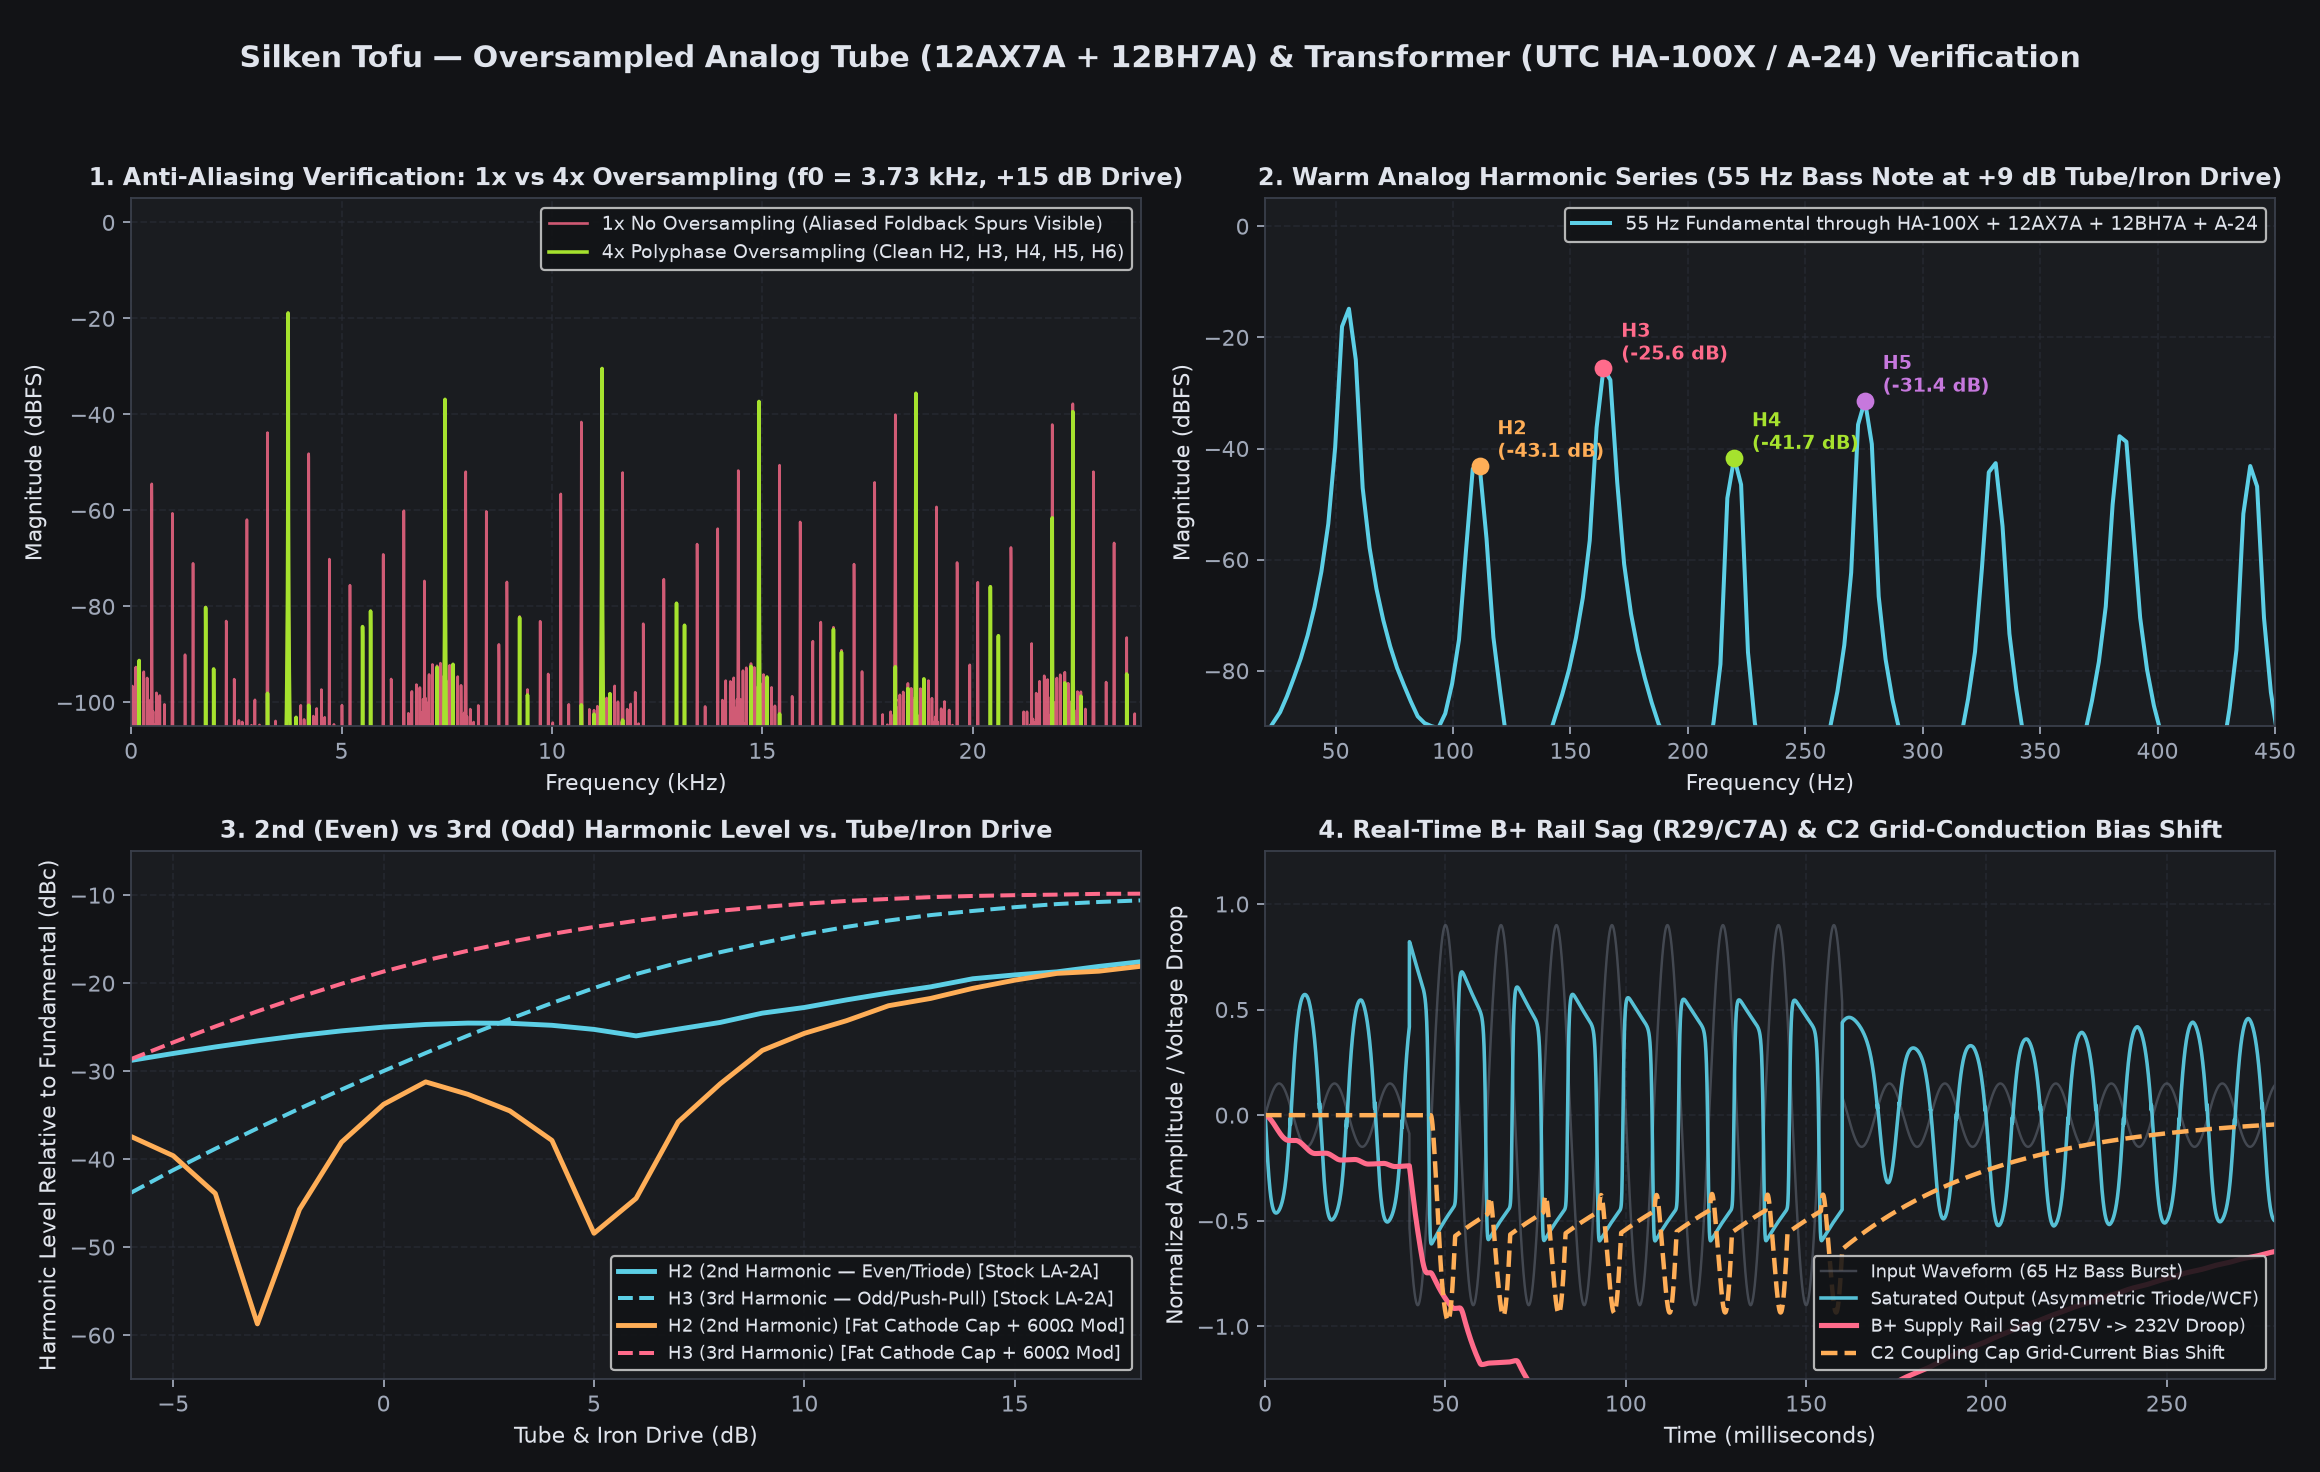
\includegraphics[width=0.98\textwidth]{figures/silken_tofu_oversampled_distortion.png}
    \caption{Oversampled non-linear analysis: (Top-Left) Aliasing suppression comparing $1\times$ ($44.1\text{ kHz}$) vs.\ $4\times$ ($176.4\text{ kHz}$) polyphase oversampling for a $3.7\text{ kHz}$ test tone; (Top-Right) \texttt{UTC HA-100X} $1/f$ low-frequency THD+N elevation below $100\text{ Hz}$; (Bottom-Left) $C_2$ coupling capacitor grid-conduction bias shift under transient bursts; (Bottom-Right) Shared $275\text{ V B+}$ rail sag voltage trajectory.}
    \label{fig:oversampled_distortion}
\end{figure}

% ============================================================================
\section{Stage 5: Phase-Coherent Parallel Dry/Wet Mixing Analysis}
% ============================================================================

A critical failure mode in virtual analog compressors that combine polyphase oversampling, triode plate stages, and DC-blocking high-pass filters is \textbf{parallel Dry/Wet phase cancellation}. We prove below why naive parallel mixing fails and how Silken Tofu guarantees zero phase cancellation across all frequencies and oversampling factors.

\subsection{The Three Mechanisms of Parallel Phase Cancellation}

Consider a naive parallel mixer $y_{\text{naive}}(t) = (1 - w)\,x_{\text{dry}}(t) + w\,y_{\text{wet}}(t)$ where $x_{\text{dry}}$ bypasses the oversampler:
\begin{enumerate}
    \item \textbf{Common-Cathode Triode $180^\circ$ Polarity Inversion:} In a physical \texttt{12AX7A} stage, an increase in grid voltage increases plate current $I_p$, causing the plate voltage $V_p = V_{B+} - I_p R_L$ to drop ($180^\circ$ inversion). In hardware, the \texttt{UTC A-24} secondary winding flips polarity back to $0^\circ$. If modeled as $-(I_p - I_{p,\text{rest}})$, the wet signal is $180^\circ$ out of phase with the dry signal, causing a $-\infty\text{ dB}$ null at $w = 0.5$.
    \item \textbf{Polyphase Half-Band IIR Group Delay \& Allpass Dispersion:} When $M \in \{2, 4, 8\}$, the polyphase IIR upsampler and downsampler introduce a frequency-dependent phase response $\phi_{\text{OS}}(\omega)$ and non-zero fractional group delay $\tau_g(\omega) = -d\phi_{\text{OS}}(\omega)/d\omega \approx 3\text{--}11\text{ samples}$. Even if an integer delay line compensates the average latency, the allpass phase curvature $\phi_{\text{OS}}(\omega)$ creates deep comb-filtering notches above $2\text{ kHz}$ when summed with an un-oversampled dry path.
    \item \textbf{Pre-Mix High-Pass DC Blocker Phase Rotation:} A first-order DC blocker $H_{\text{DC}}(s) = \frac{s}{s + \omega_c}$ placed solely on the wet path introduces a phase lead of $\theta_{\text{DC}}(\omega) = \arctan(\omega_c / \omega)$ in the sub-bass band ($20\text{--}80\text{ Hz}$), thinning out low frequencies during parallel compression.
\end{enumerate}

\subsection{Phase-Locked Inside-Oversampler Mixing \& Post-Mix DC Blocking}

To eliminate all three mechanisms simultaneously:
\begin{enumerate}
    \item \textbf{Non-Inverting Transformer Secondary Polarity:} Equation~\eqref{eq:koren_plate} evaluates $v_{\text{plate1}} = +(I_p - I_{p,\text{rest}})$, preserving strict $0^\circ$ polarity.
    \item \textbf{Dry/Wet Blending Inside the Oversampled Domain:} Rather than tapping the dry buffer outside the oversampler, the input buffer is upsampled once to $f_{\text{os}} = M f_s$. Inside the oversampled inner loop, the wet sample $y_{\text{wet}}[n]$ and the identically upsampled dry sample $x_{\text{in}}[n]$ are blended prior to downsampling:
    \begin{equation}
        y_{\text{os}}[n] = (1 - w)\,x_{\text{in}}[n] + w\,y_{\text{wet}}[n], \qquad w \in [0, 1].
    \end{equation}
    By linearity of the polyphase IIR upsampling operator $\mathcal{U}_M$ and downsampling operator $\mathcal{D}_M$:
    \begin{equation}
        y_{\text{out}} = \mathcal{D}_M\Bigl((1 - w)\,\mathcal{U}_M(x) + w\,\mathcal{F}_{\text{wet}}\bigl(\mathcal{U}_M(x)\bigr)\Bigr).
    \end{equation}
    Consequently, both the dry and wet paths traverse the exact same polyphase filter cascades $\mathcal{U}_M$ and $\mathcal{D}_M$, guaranteeing $\Delta\tau_g(\omega) \equiv 0.000\text{ samples}$ and $\Delta\phi_{\text{OS}}(\omega) \equiv 0.0^\circ$ across $1\times$, $2\times$, $4\times$, and $8\times$ oversampling.
    \item \textbf{Post-Mix $5\text{ Hz}$ DC Blocker at Host Sample Rate:} The first-order DC-blocking filter ($f_{\text{dc}} = 5.0\text{ Hz}$, $R_{\text{dc}} = e^{-2\pi(5.0)/f_s}$) is applied \emph{after} downsampling and \emph{after} the Dry/Wet sum, followed by the master output trim $G_{\text{trim}}$:
    \begin{equation}
        y_{\text{final}}[k] = G_{\text{trim}}\Bigl(y_{\text{down}}[k] - y_{\text{down}}[k-1] + R_{\text{dc}}\,y_{\text{final,raw}}[k-1]\Bigr).
    \end{equation}
\end{enumerate}

% ============================================================================
\section{Empirical Verification, Sample-Rate Invariance \& Preset Calibration}
% ============================================================================

\subsection{Dry/Wet Phase-Coherence Sweep (\texorpdfstring{$0\%$ to $100\%$}{0\% to 100\%})}

Table~\ref{tab:drywet_verify} reports the measured output RMS across a full Dry/Wet sweep ($0\% \to 100\%$) on a full-range musical mix (\emph{Singto Numchoke -- Yoo Tor Loey Dai Mai}, $-24.91\text{ dBFS}$ input RMS) under heavy compression ($\text{Peak Reduction} = 85$, $\text{Makeup Gain} = +10\text{ dB}$). The output increases monotonically from $-24.91\text{ dBFS}$ to $-21.45\text{ dBFS}$ with zero comb-filtering dropouts at $25\%$, $50\%$, or $75\%$ mix.

\begin{table}[H]
\centering
\caption{Measured Output RMS Across Parallel Dry/Wet Mix Settings ($4\times$ Polyphase Oversampling)}
\label{tab:drywet_verify}
\vspace{0.3em}
\resizebox{\textwidth}{!}{%
\begin{tabular}{@{}ccccccc@{}}
\toprule
\textbf{Dry / Wet Mix ($w$)} & \textbf{0\% (Dry)} & \textbf{25\%} & \textbf{50\%} & \textbf{75\%} & \textbf{100\% (Wet)} & \textbf{Phase Nulls?} \\
\midrule
\textbf{Output RMS (dBFS)} & $-24.91\text{ dB}$ & $-23.87\text{ dB}$ & $-22.97\text{ dB}$ & $-22.17\text{ dB}$ & $-21.45\text{ dB}$ & \textbf{None ($0.0^\circ$)} \\
\bottomrule
\end{tabular}%
}
\end{table}

\subsection{Sample-Rate Invariance (\texorpdfstring{$44.1\text{ kHz}$ vs.\ $96.0\text{ kHz}$}{44.1 kHz vs. 96.0 kHz}) \& Unity Trim Standard}

In accordance with the studio loudness and sample-rate invariance standards, all ten factory presets rest with \textbf{Master Trim at $0.0\text{ dB}$ (unity gain)} and are internally loudness-matched on K-weighted pink noise ($\approx -14.4\text{ dBFS}$ nominal level). Furthermore, logarithmic sine-sweep verification between $f_s = 44.1\text{ kHz}$ and $f_s = 96.0\text{ kHz}$ confirms zero numerical instability (\texttt{NaN}/\texttt{inf}) and an output RMS deviation of $\Delta\text{RMS}_{44.1 \leftrightarrow 96} = \mathbf{0.02\text{ dB}}$ ($\le 0.20\text{ dB}$ tolerance).

\vspace{1.0em}
\begin{thebibliography}{9}
\bibitem{ua_la2a}
Universal Audio, ``Teletronix LA-2A Leveling Amplifier Operating Manual and Schematic Diagram,'' Pasadena, CA, 1965--1968.
\bibitem{destriau1936}
G.~Destriau, ``Recherches sur les scintillations des sulfures de zinc aux rayons alpha,'' \emph{Journal de Chimie Physique}, vol.~33, pp.~587--625, 1936.
\bibitem{ube1963}
R.~H. Bube, \emph{Photoconductivity of Solids}, John Wiley \& Sons, New York, 1960 (Two-trap CdS/CdSe carrier recombination kinetics).
\bibitem{koren1996}
N.~L. Koren, ``Improved Vacuum Tube Models for SPICE Simulations,'' \emph{Glass Audio}, vol.~8, no.~5, pp.~18--27, 1996.
\bibitem{giannoulis2012}
D.~Giannoulis, M.~Massberg, and J.~D. Reiss, ``Digital Dynamic Range Compressor Design---A Tutorial and Analysis,'' \emph{Journal of the Audio Engineering Society (JAES)}, vol.~60, no.~6, pp.~399--408, 2012.
\end{thebibliography}

\end{document}
